\documentclass[a4paper,14pt]{article}
%%%%%%%%%%%%%%%%%%%%%%%  ПАКЕТЫ  %%%%%%%%%%%%%%%%%%%%%%%%%%%%%%%%%%%%%%%%%%%%%%
\usepackage{cmap}                               % Чтобы в PDF работал человеческий поиск
\usepackage[X2,T2A]{fontenc}                    % T2A = русская кодировка. X2 = яти
\usepackage[utf8]{inputenc}                     % Ввод в универсальной кодировке
\usepackage{setspace,soulutf8}      		        % Чтобы можно было менять межстрочный и межбуквенный интервалы
\usepackage{amsmath,amsfonts,amssymb,amsthm}    % Символы для математики
\usepackage{mathrsfs}                           % Символы для математики
\usepackage{dsfont}                             % Шрифт для полей действительных, комплексных... чисел командой \mathds
\usepackage[subfigure]{tocloft}  % Многоточие в оглавлении
\usepackage{array,multicol,multirow,bigstrut}   % Чтобы можно было делать в таблице колонки фиксированной ширины, слитные ячейки, вставлять strut'ы.
\usepackage{indentfirst}                        % Абзацный отступ везде
\usepackage[british,russian]{babel}             % Русские переносы, тире, типографика, самодержавие, духовность!
\usepackage[perpage]{footmisc}                  % Сброс счётчика сносок на каждой странице
\usepackage[pdftex,unicode,bookmarks=true,bookmarksopen=true,colorlinks=true,linkcolor=blue,urlcolor=blue,citecolor=blue]{hyperref} % Синие ссылки в PDF
\usepackage{microtype}                          % Свешивающаяся пунктуация и подгонка белого пространства по правилу \pm 2 процента
\usepackage{textcomp}                           % Чтобы в формулах можно было русские буквы писать через \text{}
\usepackage[paper=a4paper,top=12.7mm, bottom=12.7mm,left=12.7mm,right=12.7mm,bindingoffset=6.6mm,includefoot]{geometry} % Достаточно экономные размеры листа и поля для нумерации страниц внизу (для колонтитулов в стиле лекций по матану, нужно includefoot заменить на includehead и не только
\usepackage{xcolor}                             % Чтобы можно было цветные объекты вставлять
\usepackage[pdftex]{graphicx}                   % Чтобы вставились изображения
\usepackage{float,longtable}                    % Поддержка плавающих таблиц и рисунков
\usepackage[margin=0pt,font=small,labelfont=bf,labelsep=period]{caption} % Подписи таблиц и рисунком мелкие, жирные, с принятым в русской типографике разделителем.
\usepackage{rotating}                           % Создание своих акцентов, поворот объекта.
\usepackage{datetime}                           % Отображение времени
%\usepackage{embedfile}                         % Чтобы код LaTeXа включился как приложение в PDF-файл
\usepackage{xspace}
\usepackage{wrapfig,enumitem}                   % Обтекаемые текстом рисунки
\usepackage{mathtools}                          % В тексте используется smashoperator, чтобы избежать некрасивых пробелов вокруг сумм и пределов с большим подстрочником
\usepackage{cancel}                             % Красивое <<вычёркивание>> сокращающихся выражений одноимённой командой
\usepackage{tikz,pgfplots}			% Рисование графиков непосредственно кодом
\usepackage{subfigure}
\usepackage{fancyhdr}	% Пакет для создания колонтитулов в стиле лекций по матану
\usepackage{accents}
\usepackage{pb-diagram}

%%%%%%%%%%%%%%%%%%%%%%%  ПАРАМЕТРЫ  %%%%%%%%%%%%%%%%%%%%%%%%%%%%%%%%%%%%%%%%%%%
\setstretch{1}                          % Межстрочный интервал
\flushbottom                            % Эта команда заставляет LaTeX чуть растягивать строки, чтобы получить идеально прямоугольную страницу
\righthyphenmin=2                       % Разрешение переноса двух и более символов
\pagestyle{plain}                       % Нумерация страниц снизу по центру.
\settimeformat{hhmmsstime}              % Формат времени с секундами
\widowpenalty=300                       % Небольшое наказание за вдовствующую строку (одна строка абзаца на этой странице, остальное --- на следующей)
\clubpenalty=3000                       % Приличное наказание за сиротствующую строку (омерзительно висящая одинокая строка в начале страницы)
\setlength{\parindent}{1.5em}           % Красная строка.
\setlength{\topsep}{0pt}                % Уничтожение верхнего отступа, если он где проявится
%%%%%%%%%%%%%%%%%%%%%%%%%%%%%%%%%%%%%%%%%%%%%%%%%%%%%%%%%%%%%%%%%%%%%%%%%%%%%%%

%%%% Техническая подготовка для определения следующих команд %%%%
\makeatletter
\newcommand*{\relrelbarsep}{.386ex}
\newcommand*{\relrelbar}{%
  \mathrel{%
    \mathpalette\@relrelbar\relrelbarsep
  }%
}
\newcommand*{\@relrelbar}[2]{%
  \raise#2\hbox to 0pt{$\m@th#1\relbar$\hss}%
  \lower#2\hbox{$\m@th#1\relbar$}%
}
\providecommand*{\rightrightarrowsfill@}{%
  \arrowfill@\relrelbar\relrelbar\rightrightarrows
}
\providecommand*{\leftleftarrowsfill@}{%
  \arrowfill@\leftleftarrows\relrelbar\relrelbar
}
\providecommand*{\xrightrightarrows}[2][]{%
  \ext@arrow 0359\rightrightarrowsfill@{#1}{#2}%
}
\providecommand*{\xleftleftarrows}[2][]{%
  \ext@arrow 3095\leftleftarrowsfill@{#1}{#2}%
}
\makeatother



%%%%%%%%%%%%%%%%%%%%% Команды-сокращения %%%%%%%%%%%%%%%%%%%%%%%%%%%%%%%%%%%%%%
\newcommand{\pau}{\hskip .75em plus.1em minus.08em\relax}	% пробел для выражений с кванторами, например «\forall\ \e>0\pau\exists\ \delta\colon», где \e определяется как
\newcommand{\ds}{\displaystyle}			% Быстрое переключение на выключный стиль формулы, где интегралы и суммы большие
\newcommand{\e}{\varepsilon}                % эпсилон
\newcommand{\p}{\partial}                   % частная производная
\renewcommand{\phi}{\varphi}                % Чтоб фи писалась в соответствии с русской традицией
\newcommand{\q}{\varnothing}			% Пустое множество в русской традиции
\newcommand{\N}{\mathds{N}}			% Натуральные числа
\newcommand{\Z}{\mathds{Z}}			% Целые числа
\newcommand{\Q}{\mathds{Q}}			% Рациональные числа
\newcommand{\R}{\mathds{R}}			% Действительные числа
\renewcommand{\C}{\mathds{C}}			% Комплексные числа
\newcommand{\T}{\mathbb{T}}			% Отмеченное разбиение (для интегральных сумм Римана или Римана"--~Стилтьеса
\newcommand{\Rim}{\mathcal R}			% Риман
\renewcommand{\le}{\leqslant}           % Правильное меньше или равно
\renewcommand{\leq}{\leqslant}           % Правильное меньше или равно
\renewcommand{\ge}{\geqslant}           % Правильное больше или равно
\renewcommand{\geq}{\geqslant}           % Правильное больше или равно
\newcommand{\dd}{\setminus}		% Ассоциируется с diagdown, но это именно вычитание множеств
\renewcommand{\iff}{\,\Leftrightarrow\,}	% Если и только если
\newcommand{\imp}{\hspace{1pt plus1pt}\Rightarrow\hspace{1pt plus1pt}}		% Следовательно
\def\hm#1{#1\nobreak\discretionary{}{\hbox{$#1$}}{}} % Команда для переноса на следующую строку символов бинарных операций
\renewcommand{\a}{\langle} 		% Открывающая треугольная скобка
\newcommand{\s}{\rangle}		% Закрывающая треугольная скобка
\newcommand{\ol}[1]{\overline{#1}}	% Надчёркивание аргумента по всей ширине

%%%% СТРЕЛКИ %%%%%%%%%%%%%%
\renewcommand{\to}{\rightarrow}                   % Правильная стрелка вправо («стремится») без возможности подписать
\newcommand{\To}[1]{\xrightarrow{#1}}		% Стрелка «стремится», ширина которой зависит от ширины агрумента-подписи (подпись ставится вверху)
\newcommand{\tend}[1]{\xrightarrow[#1]{}}	% Стрелка «стремится», ширина которой зависит от ширины агрумента-подписи (подпись ставится внизу)
\newcommand{\Tot}[1]{\xrightarrow{\text{#1}}}	% Стрелка «стремится», ширина которой зависит от ширины текстового агрумента-подписи (подпись ставится вверху)
\newcommand{\te}[1][]{\xrightarrow[n\to\infty]{#1}}	% Стремится при n стремящемся к бесконечности
\newcommand{\TE}{\xrightarrow[N\to\infty]{}}	% Стремится при N стремящемся к бесконечности
\newcommand{\neV}{\overline{\vphantom{<}\quad}\kern-.35em\searrow}	% Не возрастает в стиле лекций по анализу
\newcommand{\neU}{\underline{\vphantom{<}\quad}\kern-.35em\nearrow}	% Не убывает
\newcommand{\rsh}[2][P]{\xrightrightarrows[{#2\to\infty}]{#1}}		% Двойная растяжимая стрелка «равномерно сходится последовательность». Снизу стрелки подпись-обязательный-аргумент, к которому приписывается автоматически стремление к бесконечности. Необязательные аргумент изменяет подпись сверху с P на то, что напишите
\newcommand{\rsH}[2][X]{\xrightrightarrows[{#2}]{#1}} % Равномерная сходимость по параметру. Подпись снизу задаётся явно и обязательно; подпись сверху задаётся необязательно, по умолчанию X
\newcommand{\nsh}[2][n]{\xrightarrow[#1\to\infty]{\|\ \|_{#2}}}		% Растяжимая стрелка «сходится по норме». Вид нормы подписывается в обязательном аргументе (например l_2). Необязательный аргумент «что стремится к бесконечности» (стремление к бесконечности приписывается автоматически)


%%%%% Предел как оператор %%%%%%%%
\newcommand{\yo}[2]{\lim\limits_{#1\to#2}}	% предел{при этой букве}{стремящейся сюда}
\newcommand{\prb}[1]{\lim\limits_{#1}}		% предел{по такой базе}

%%%%%% O-символика %%%%%%%%%%%%
\newcommand{\oo}{\overline{\overline o}} 		% o-малое без подписей и скобок (две черты сверху ставятся автоматически). Переопределение этой команды изменит вид всех надстроек, указанных ниже
\newcommand{\ou}{\underline{\underline{O}}}		% Аналогично O-большое
\newcommand{\ouu}[2]{\underset{#2\ }\ou(#1)}		% O-большое{по отношению к чему}{при каком процессе}
\newcommand{\ooo}[2]{\underset{#2\ }\oo(#1)} % o-малое{по отношению к чему}{при каком процессе}
\newcommand{\ooob}[2]{\underset{#2}{\oo\big(#1\big)}}	% Аналогично, только скобки вокруг первого аргумента с плавающим размером
\newcommand{\ooog}[2]{\underset{#2}{\ou\big(#1\big)}}

%%%%%% Дифференцирование %%%%%%%%%%%%%%
\newcommand{\CP}[2]{\frac{\partial #1}{\partial #2}}	% Частная производная{чего}{по чему}
\newcommand{\cP}[2]{\frac{d #1}{d #2}}			% Полная/материальная производная
\newcommand{\Jacoby}[4]{\begin{pmatrix}
\CP {{#1}_{1}}{{#2}_1} 	& \CP{{#1}_{1}}{{#2}_2} & \dots & \CP{{#1}_{1}}{{#2}_{#3}} \\[1ex]
\CP {{#1}_{2}}{{#2}_1} 	& \CP{{#1}_{2}}{{#2}_2} & \dots & \CP{{#1}_{2}}{{#2}_{#3}} \\
\vdots 			& \vdots		& \ddots& \vdots \\
\CP {{#1}_{#4}}{{#2}_1} & \CP{{#1}_{#4}}{{#2}_2}& \dots & \CP{{#1}_{#4}}{{#2}_{#3}}	
\end{pmatrix}}% матрица Якоби{чего}{по чему}{размерность образа}{размерность аргумента}


\newcommand{\ttilde}[1]{\tilde{\tilde{#1}}}	% Набрать символ(ы)-аргумент с двумя узкими волнами
\newcommand{\Til}[1]{\widetilde{#1}{} }		% Набрать символ(ы)-аргумент с волной, ширина которой равна ширине аргумента

%%%% ПОСЛЕДОВАТЕЛЬНОСТИ, СУММЫ, ПРОИЗВЕДЕНИЯ %%%%%
\newcommand{\pos}[2][n]{\big\{{#2}_{#1}\big\}_{#1=1}^\infty} 		% Последовательность: в фигурных скобках аргумент с нижним индексом по умолчанию n; справа от скобок подпись n (или необязательный аргумент) от 1 до бесконечности
\newcommand{\ar}[4]{\big\{{#1}_{#2}\big\}_{#2=#3}^{#4}} % Задание последовательности четырьмя аргументами: что, каким символом нумеруется, откуда, докуда
\newcommand{\Har}[4]{\left\{{#1}_{#2}\right\}_{#2=#3}^{#4}} % Аналог предыдущего, но размер фигурных скобок подстраивается под внутренность.
\newcommand{\AR}[3]{\big\{#1\big\}_{#2}^{#3}} 		% Последовательность. Три аргумента: {что и как нумеруеся}{номер=начальное значение}{конечное значение номера}
\newcommand{\ry}[3][1]{\sum\limits_{{#3}={#1}}^\infty {#2}_{#3}}	% Ряд[с какого номерая начиная]{чего}{как нумеруется}; по умолчанию с единицы; Например, \ry an
\newcommand{\rY}[2][1]{\sum\limits_{{#2}={#1}}^\infty} % Сумма до бесконечности[с какого номера начать]{символ индекса}; например, \rY n или \rY[0]j
\newcommand{\RY}[3]{\sum\limits_{#1 = #2}^{#3}}		% Сумма{по этому индексу}{от этого значения индекса}{до этого значения индекса}; Например, \RY n1N
\newcommand{\tmy}[3][1]{\prod\limits_{#3=#1}^{\infty}#2_{#3}}	% Бесконечное произведение (от слова times), аналог \ry
\newcommand{\tmY}[2][1]{\prod\limits_{#2=#1}^{\infty}} % аналог \rY
\newcommand{\TMY}[3]{\prod\limits_{#1=#2}^{#3}}		% аналог \RY



%%%%% Окружения для нумерованных перечней
\newenvironment{iItems}{\begin{enumerate}\let\AEtheenumi\theenumi{}\renewcommand{\theenumi}{\roman{enumi}}\renewcommand{\labelenumi}{(\theenumi)}}{\renewcommand{\labelenumi}{\theenumi.}\renewcommand{\theenumi}{\AEtheenumi}\end{enumerate}}	% (i), (ii), ...
\newenvironment{azItems}{\begin{enumerate}\let\AEtheenumi\theenumi{}\renewcommand{\theenumi}{\asbuk{enumi}}\renewcommand{\labelenumi}{(\theenumi)}}{\renewcommand{\labelenumi}{\theenumi.}\renewcommand{\theenumi}{\AEtheenumi}\end{enumerate}}	% (а), (б), ...
\newenvironment{roItems}{\begin{enumerate}\renewcommand{\labelenumi}{(\theenumi)}}{\renewcommand{\labelenumi}{\theenumi.}\end{enumerate}}	% (1), (2), ...
\newenvironment{oItems}{\begin{roItems}\setcounter{enumi}{-1}}{\end{roItems}}	% (0), (1), ...
%%% В КОНЦЕ ФАЙЛА ПРИВЕДЕНЫ КОМАНДЫ, КОТОРЫЕ Я НЕ УСПЕЛ ОПИСАТЬ

%%%%%%%%%%%%%%%%%%%% Операторы в смысле LaTeX %%%%%%%%%%%%%%%%%%%%%%%%%%%%%%%%%
\DeclareMathOperator{\sign}{sgn}	% Знак (перестановки)
\DeclareMathOperator{\sgn}{sgn}		% Сокращённая альтернатива sign
\DeclareMathOperator{\diag}{diag}	% Диагональная матрица
\DeclareMathOperator{\const}{const}	% Константа
\DeclareMathOperator{\rang}{rank}         % Оператор ранга
\DeclareMathOperator{\rank}{rank}	% На любой вкус
\DeclareMathOperator{\diam}{diam}	% Диаметр, например, разбиения
\DeclareMathOperator{\card}{card}	% Мощность множества
\DeclareMathOperator{\osc}{osc}		% Осцилляция	
\DeclareMathOperator{\grad}{grad}	% Градиент
\DeclareMathOperator{\intS}{int}	% Внутренность множества
\DeclareMathOperator{\ext}{ext}		% Внешность множества
\DeclareMathOperator{\supp}{supp}
\DeclareMathOperator{\extr}{extr}


%%%%%%% Математическая экзотика %%%%%
\newcommand{\defequiv}{\mathbin{\vbox{\baselineskip=1.95pt\lineskiplimit=0pt\hbox{.}\hbox{.}\hbox{.}}\hskip-0.3em\equiv}} 		% вертикальное троеточие =, то есть «по определению тождественно»
\newcommand{\rus}[1]{\mbox{\rm{\scriptsize{#1}}}}	% команда убивает зависимость русского текста в формуле от стиля абзаца (но и от стиля формулы тоже). Специально для обозначения левой и правой производных, чтобы  f'_п печаталось с прямой буквой «п» и нельзя было спутать с n
\newcommand{\overcirc}[1]{\accentset{\circ}{#1}}	% круг над символом
\newcommand{\overstar}[1]{\accentset{\bigstar}{#1}}	% звезда над символом

%%%%%%%%%%%%%%%%%%% Глобальные текстовые команды %%%%%%%%%%%%%%%%%%%%%%%%%%%%%%
\newcommand{\ENGs}[1]{\foreignlanguage{british}{#1}} % Переключение правил переноса и прочих правил автооформления на английский язык действует на аргумент
\newcommand{\ENG}{\selectlanguage{british}} % Глобальное переключение (если просто начать писать на другом язык, велика вероятность появления очень больших пробелов или помещения части слова за границу листа
\newcommand{\RUS}{\selectlanguage{russian}}
\newcommand{\fnnsp}{\hspace{-0.4em}} % Знак сноски принято ставить до всех знаков препинания, кроме ! ? ...
% А если есть возможность подвинуть низкий знак препинания под сноску, то для этого Андрей Викторович и придумал \fnnsp
\let\myfootnote\footnote
\renewcommand{\footnote}[1]{\myfootnote{\;#1}} % Сноски Андрея Виторовича

%%%%%%%% Определение разрядки разреженного текста и задание красивых и притом регулируемых многоточий
% Зачем и почему описано в блоге http://kostyrka.ru/blog
\newdimen\ellipsiskern
\setlength{\ellipsiskern}{.1em}
\newdimen\ellipsiskernen
\setlength{\ellipsiskernen}{.2em}
\newcommand{\ldotst}{.\kern\ellipsiskern.\kern\ellipsiskern.}	% вместо ... пишем \ldotst{}
\newcommand{\ldotse}{!\kern\ellipsiskern.\kern\ellipsiskern.}	% вместо !.. пишем \ldotse{}
\newcommand{\ldotsq}{?\kern\ellipsiskern\kern-.11em.\kern\ellipsiskern.}	% вместо ?.. пишем \ldotsq{}
\newcommand{\ldotsten}{.\kern\ellipsiskernen.\kern\ellipsiskernen.}		% аглийское ...
\newcommand{\ldotspen}{.\kern\ellipsiskernen.\kern\ellipsiskernen.\kern\ellipsiskernen\kern.15em.}
\newcommand{\ldotseen}{.\kern\ellipsiskernen.\kern\ellipsiskernen.\kern\ellipsiskernen\kern.15em!}
\newcommand{\ldotsqen}{.\kern\ellipsiskernen.\kern\ellipsiskernen.\kern\ellipsiskernen\kern.067em?}
%%%%%%%%%%%%%%%%%%%%%%%%%%%%%%%%%%%%%%%%%%%%%%%%%%%%%%%%%%%%%%%%%%%%%%%%%%%%%%%



%%%%%%%%%%%%%%%%%%%%%%% ДРУГИЕ ПОЛЕЗНЫЕ КОМАНДЫ БЕЗ КОММЕНТАРИЕВ (ПОКА) %%%%%%%
\newcounter{rad}
\setcounter{rad}{1}
% a_1+a_2+\ldots
	\def\rad#1#2{\ifnum \therad < \the\numexpr(#2 + 1)\relax #1_\therad + \addtocounter{rad}{1} \rad{#1}{#2}\else \ldots \fi \setcounter{rad}{1}}
%a_{N+1}+a_{N+2}+\ldots
	\def\raD#1#2#3{\ifnum \therad < \the\numexpr(#2 + 1)\relax #1_{#3{\therad}} + \addtocounter{rad}{1} \raD{#1}{#2}{#3}\else \ldots \fi \setcounter{rad}{1}}
\def\crad#1#2#3#4{\ifnum \therad < \the\numexpr(#4 + 1)\relax #1{\therad}#3 + \addtocounter{rad}{1} \crad{#1}{#2}{#3}{#4}\else \ldots +#1{#2}#3 \fi \setcounter{rad}{1}}
\def\craD#1#2#3#4#5#6{\ifnum \therad < \the\numexpr(#4 + 1)\relax #1{#5{\therad}#6}#3 + \addtocounter{rad}{1} \craD{#1}{#2}{#3}{#4}{#5}{#6}\else \ldots +#1{#5#2#6}#3  \fi \setcounter{rad}{1}}
%repeat argument #1 #2 times
	\def\tfT#1#2{\ifnum \therad < \the\numexpr(#2 + 1)\relax #1\addtocounter{rad}{1} \tfT{#1}{#2}\else \fi \setcounter{rad}{1}}
\def\dI#1#2#3#4#5#6{\ifnum \therad < \the\numexpr(#6 + 1)\relax {#1}_{\therad}{#3}_{\therad}#5\addtocounter{rad}{1} \dI{#1}{#2}{#3}{#4}{#5}{#6}\else \dots #5{#1}_{#2}{#3}_{#4}\fi \setcounter{rad}{1}}
\def\DI#1#2#3#4#5#6{\ifnum \therad < \the\numexpr(#6 + 1)\relax #1\therad#3\therad#5\addtocounter{rad}{1} \DI{#1}{#2}{#3}{#4}{#5}{#6}\else \dots #5#1#2#3#4\fi \setcounter{rad}{1}}
\def\iSum#1#2#3{\ifnum \therad < #3\relax {#1}_{\therad}{#2}_{\the\numexpr(#3 - \therad + 1)\relax}+ \addtocounter{rad}{1}\iSum{#1}{#2}{#3}\else {#1}_{\therad}{#2}_{1}\fi \setcounter{rad}{1}}
\def\tms#1#2{\ifnum \therad < \the\numexpr(#2 + 1)\relax #1_\therad \ifnum \therad < \the\numexpr(#2)\relax \cdot \else \fi\addtocounter{rad}{1} \tms{#1}{#2}\else \cdots \fi \setcounter{rad}{1}}
\def\ctms#1#2#3#4#5{\ifnum \therad < \the\numexpr(#4 + 1)\relax #1{#2\therad}#3 \ifnum \therad < \the\numexpr(#4)\relax \cdot \else \fi\addtocounter{rad}{1} \ctms{#1}{#2}{#3}{#4}{#5}\else \cdots #1{#2#5}#3\fi \setcounter{rad}{1}}
\newcommand{\cSize}{\footnotesize}
\newcommand{\cmt}[1]{\text{\cSize #1}}
\newcommand{\BIggl}[1]{\left#1\vphantom{\Bigg(\frac12\Bigg)^2}\right.}
\newcommand{\BIggr}[1]{\left.\vphantom{\Bigg(\frac12\Bigg)^2}\right#1}


\input{all/my.sty}
\usepackage{caption}
\usepackage{pdfpages}


\begin{document}
\begin{titlepage}
\thispagestyle{empty}
\setcounter{page}{0}
\begin{center}{
\Large Московский государственый университет 

им. М.",В.",Ломоносова

Механико-математический факультет

Кафедра газовой и волновой динамики}
\end{center}
\vspace{120pt}
\begin{center}
\Large Ракитин Виталий Павлович.
\end{center}
\vspace{20pt}
\begin{center}{\LARGE Численное решение краевой задачи принципа максимума в задаче оптимального управления методом стрельбы.}
\end{center}

\vspace{80pt}
%\begin{flushleft}
%{\largeНаучный руководитель:

%\vspace{6pt}
%чл.-корр. РАН, проф. Трещев Д.",В.}
%\end{flushleft}
\vfill
\begin{center}
Москва, 2015 год.
\end{center}
\end{titlepage}
\tableofcontents
\newpage
\section{Постановка заадачи}

Рассматривается задача (номер 34) Лагранжа с фиксированным временным отрезком, без ограничений вида <<меньше или равно>>:

\begin{eqnarray}\label{task}
\int\limits_{0}^{1} \frac{\ddot{x}^2}{1 + \alpha t^2x^2} dt &\to& \extr, \\
\int\limits_{0}^{1} xdt &=&  1\notag,\\
\qquad x(0) = \dot{x}(1) &=&  0\notag,\\
\dot{x}(0) &=&  1\notag,
\end{eqnarray}
где $\alpha$ "--- известная константа, параметр задачи.

Требуется формализовать задачу как задачу оптимального управления, принципом максимума
Понтрягина свести задачу к краевой задаче, численно решить полученную краевую задачу методом стрельбы и обосновать точность полученных результатов, проверить полученные экстремали Понтрягина на оптимальность при~различных значениях параметра 
\[ \alpha = \{0.0;\quad 0.1; \quad 1.0; \quad 10.0\}.\]

\section{Формализация задачи}
Формализуем задачу для оптимального управляения. Для этого введём следующие обозначения
\[
y = \dot{x}, \qquad u = \dot{y} = \ddot{x}.
\]
где $u$ "--- управление. 

Тогда исходная система~(\ref{task}) перепишется в виде:
\begin{equation}\label{formtask}
	\begin{cases}
		\dot{x} = y;\\
		\dot{y} = u;\\
		u \in \R;\\
		x(0) = 0, \quad y(0) = 1;\\
		y(1) = 0;\\
		\int\limits_{0}^{1} xdt = 1;\\
		\int\limits_{0}^{1} \frac{u^2}{1 + \alpha t^2x^2} dt \to extr.\\
	\end{cases}
\end{equation}

\section{Система необходимых условий оптимальности}

Рассмотртим задачу Лагранда в пространстве $\Omega = C^1(\Delta, \R^2)\times C(\Delta, \R)\times \R^2$:
\[
u(t) \in \R, \qquad
\ol{x}^T = (x,y) \in \R^2,\qquad 
\dot{\ol{x}}^T - (y,u) = 0, \qquad 
\phi(t,\ol{x}(t),u(t)) = (y,u);
\]
Далее выпишем следующий функционалы
\[
B_i(\ol{x},u,t_0,t_1) = B_i(x,y,u,0,1) =  \int\limits_0^1 f_i(t,\ol{x},u)dt + \psi_i(0,\ol{x}(0),1,\ol{x}(1)), \qquad \text{где }i = 1,\dots,4.
\]
\[
B_0 =  \int\limits_0^1 \frac{u^2}{1 + \alpha t^2} dt, \qquad f_0 = \frac{u^2}{1 + \alpha t^2}, \qquad
\psi_0 = 0;
\]
\[
B_1 =
\int\limits_0^1 xdt - 1 = 0, \qquad
f_1 = x, \qquad \psi_1 = -1;
\]
\[
B_2 = x(0), \qquad f_2 = 0, \qquad \psi_2 = x(0);
\]
\[
B_3 = y(0) - 1, \qquad f_3 = 0, \qquad \psi_3 = y(0) - 1 ;
\]
\[
B_4 = y(1), \qquad f_4 = 0, \qquad \psi_4 = y(1);
\]

Далее выпишем функцию Лагранжа
\[
\mathcal{L} = \int\limits_{0}^{1} L dt + l;
\]
где
\[
\text{лагранжиан: }
L = \sum\limits_{i=0}^{4} \lambda_i f_i(t,\ol{x},u) + \langle \ol{p}(t),\dot{\ol{x}} - \phi(t,\ol{x},u)\rangle;
\]
\[
\text{терминант: }
l = \sum\limits_{i=0}^{4} \lambda_i \psi_i(0,\ol{x}(0),1,\ol{x}(1));
\]
\[
\lambda = \left(\lambda_0, \dots, \lambda_4 \right), \qquad
\ol{p}(\cdot) = (p_x,p_y)  \in C^1(\Delta, \R^{2*})
\]
множетели лагранжа задачи, а так же функцию Понтрягина
\[
H(t,\ol{x},u,\ol{p},\lambda) = \langle \ol{p}(t), 
\phi(t,\ol{x},u)\rangle - \sum\limits_{i=0}^{4}\lambda_i f_i(t,\ol{x},u). 
\]

А теперь выпишем функции Лагранжа и Понтрягина в явном виде:
\begin{equation}
L = \lambda_0 \left(\frac{u^2}{1 + \alpha t^4}\right) +\lambda_1 x+ p_x (\dot x - y)
+ p_y (\dot y - u);
\end{equation}
\[
l = -\lambda_1 + \lambda_2 x(0) + \lambda_3(y(0) - 1) + \lambda_4 y(1);
\]
\[
H = p_x y + p_y u - \lambda_0 \left(\frac{u^2}{1 + \alpha t^4}\right) - \lambda_1 x;
\]

Далее применим к задаче оптимального управления~(\ref{formtask}) принцип максимума Понтрягина. Необходимые условия оптимальности:
\begin{enumerate}
\item Уравнения Эйлера-Лагранжа (сопряжённая система уравнений, условие стационарности по $\ol{x}$):
\begin{equation}\label{Euler}
\begin{cases}
\dot {p}_x = - \frac{\partial H}{\partial x} = \lambda_1;\\
\dot {p}_y =  - \frac{\partial H}{\partial y} = -p_x.
\end{cases}
\end{equation}
\item\label{optimal}
условие оптимальности по управлению,
\[
u = \mathrm{arg} \mathop{\rm abs}\limits_{u \in \R} \max H(u) = \mathrm{arg} \mathop{\rm abs}\limits_{u \in \R} \max \left(p_y u - \left(\frac{\lambda_0}{1+\alpha t^4}\right)  u^2\right) = \frac{p_y \left(1+\alpha t^4\right)}{2\lambda_0}
\]
при $\lambda_0 \not= 0$, так как $H(u)$ "--- парабола, с ветвями, направленными вниз (т.к. $\lambda_0 \ge 0$
"--- см.п.~\ref{notzero}), достигает максимума в вершине, при указанном значении аргумента $u$;
\item\label{trans}
условия трансверсальности по $\ol{x}$:
\[
p_x(t_k) = (-1)^k \frac{\partial l}{\partial x(t_k)}, \qquad
p_y(t_k) = (-1)^k \frac{\partial l}{\partial y(t_k)}. \qquad
\]
В нашем случае $k = 0, 1$, $t_0 = 0$, $t_1 = 1$. Значит
\[
p_x(0) = \lambda_2,
\qquad
p_x(1) = 0,
\qquad
p_y(0) = \lambda_3,
\qquad
p_y(1) = - \lambda_4. 
\] 
\item условия стационарности по $t_k$:\\ нет, так как в задаче~(\ref{formtask}) $t_k$ "--- известные константы;
\item условия дополняющей нежёсткости:\\ нет, так как в задаче~(\ref{formtask}) отсутствуют условия вида <<меньше или равно>>;
\item\label{notzero}
условие неотрицательности: $\lambda_0 \ge 0$;
\item условие нормировки (множители Лагранжа могут быть выбраны с точностью до положительного множителя);
\item\label{NERON}
НЕРОН (множители Лагранжа НЕ Равны Одновременно Нулю).
\end{enumerate}
\section{Анормальный случай и исследование задачи}
Исследуем возможность анормального случая $\lambda_0 = 0$. При  $\lambda_0 = 0$ из (\ref{formtask}) и (\ref{Euler}) получим систему дифференциальных уравнений:
\begin{equation}
	\begin{cases}
	\dot{x} = y;\\
	\dot{y} = u;\\
	\dot{p}_x = \lambda_1;\\
	\dot{p}_y = -p_x;
	\end{cases}
\end{equation}

Отсюда получаем, 
\[
p_x(t) = \lambda_1 t + C, \qquad p_y(t) = - \lambda_1 t - C. 
\]
Так же из условия (п.~\ref{optimal}), имеем 
\[
p_y(t) \equiv 0, \qquad
\dot{p}_y(t) \equiv 0,
\] 
иначе 
\[
u(t) = \pm \infty,
\] 
и такой управляемый процесс не является допустимым. Следовательно, 
\[
\lambda_1 t + C = 0,\qquad
\lambda_1 t = C, \qquad 
\]
где $t \in \R$, $\lambda_1, C = \mathrm{const}$, тогда
\[
\lambda_1 = C = 0, \qquad
p_x(t) \equiv 0.
\]
Из условий трансверсальности (п.~\ref{trans}) получаем 
\[
\lambda_1 = \lambda_2 = \lambda_3 = \lambda_4 = 0. 
\]
Таким образом, если $\lambda_0 = 0$, то все множители Лагранжа равны $0$ и получается противоречие с условием (п.~\ref{NERON}). Значит, анормальный случай невозможен.

Так как $\lambda_0 \not= 0$, то в силу однородности функции Лагранжа по множителям Лагранжа выберем следующее условие нормировки:
\[
\lambda_0 = \frac{1}{2},
\]
тогда из условия (п.~\ref{optimal}) определяется управление
\begin{equation}
u = p_y (1 + \alpha t^2x^2), 
\end{equation}
%\[
%\text{где } \alpha = \{0.0;\quad 0.1; \quad 1.0; \quad 10.0\},\quad 
%t \in [0,1]. 
%\]

\section{Краевая задача}
Ко всему вышесказанному добавим, что 
\[
\int\limits_{0}^{1} x dt = 1.
\]
Введём обозначение
\[
\phi(t) = \int\limits_{0}^{1} x(\tau) d\tau, \quad \text{а так же } \lambda_1 = a;
\]
тогда 
\begin{equation}\label{dopeqq}
\begin{cases}
\phi(0) = 0,\\ 
\dot\phi = x;\\
\phi(1) = 1;
\end{cases}
\end{equation}

Таким образом, на основе принципа максимума Понтрягина задача оптимального управления~(\ref{formtask}) сводится к~краевой задаче~(\ref{finaltask}). 
\begin{equation}\label{finaltask}
	\begin{cases}
	\dot{x} = y; \\
	\dot{y} = p_y (1 + \alpha t^4);\\ %т.к. \dot{y} = u
	\dot{p}_x = \lambda_1 = a; \\
	\dot{p}_y = - p_x;\\
	\dot\phi = x;\\
	\dot{a} = 0.
	\end{cases}
\end{equation}
\[
	x(0) = 0, \qquad y(0) = 1, \qquad \phi(0) = 0;
\]
\[
 	y(1) = 0, \qquad p_x(1) = 0. \qquad \phi(1) = 1;
\]
\[ \alpha = \{0.0;\quad 0.1; \quad 1.0; \quad 10.0\}.\]

Однако, $\lambda_1$ в краевой задаче

\section{Аналитическое решение краевой задачи}
Полученная краевая задача решается аналитически.
\begin{enumerate}
\item из уравнения $\dot{p}_x = 1$ следует, что 
\[
p_x = t + C_1,
\] 
где $C_1 = \mathrm{const}$.\\
Так же из краевых условий видим, что $p_x(1) = 0$, тогда $0 = 1 + C_1$, значит $C_1 = -1$.
\item из уравнения 
\[
\dot{p}_y = - p_x = - t + 1
\]
 получим, что 
 \[
 p_y = -\frac{1}{2} t^2 + t + C_2,
 \qquad 
\text{где } C_2 = \mathrm{const}.
\]
\item  из уравнения 
\[
\dot{y} = p_y (1 + \alpha t^4) = (-\frac{1}{2} t^2 + t + C_2)(1 + \alpha t^4)
\]
 не сложно получить, 
\[
y = \frac{1}{2} \left(-\frac{2}{5} \alpha C_2 t^5-\frac{\alpha t^7}{7}-\frac{\alpha t^6}{3}-2 C_2 t-\frac{t^3}{3}-t^2\right)+C_3
\]
Из краевых условий $y(0) = 1$, $y(1) = 0$ получим
\[
C_3 = 1, \qquad C_2 = -\frac{5 (5 \alpha -7)}{21 (\alpha + 5)}.
\]
А значит 
\[
y = \frac{1}{42} \left(t \left(t \left(-3 \alpha t^5-7 \alpha t^4+\frac{2 \alpha(5 \alpha-7) t^3}{\alpha + 5}-7 t-21\right)-\frac{320}{\alpha + 5}+50\right)+42\right)
\]
\item из уравнения 
\[
\dot{x} = y = \frac{1}{42} \left(t \left(t \left(-3 \alpha t^5-7 \alpha t^4+\frac{2 \alpha(5 \alpha-7) t^3}{\alpha + 5}-7 t-21\right)-\frac{320}{\alpha + 5}+50\right)+42\right)
\]
следует
\[
x = \frac{t}{1008} \left(-9 \alpha t^7-24 \alpha t^6+\frac{8 \alpha (5 \alpha-7) t^5}{\alpha+5}+\frac{120 (5 \alpha-7) t}{\alpha+5}-42 t^3-168 t^2+1008\right) + C_4,
\]
Из краевых условий $x(0) = 0$, тогда
\[
C_4 = 0
\]
\end{enumerate}

Из вышесказанного следует, что решением нашей системы будет следующим
\[
	\begin{cases}
	x = \frac{t}{1008} \left(-9 \alpha t^7-24 \alpha t^6+\frac{8 \alpha (5 \alpha-7) t^5}{\alpha+5}+\frac{120 (5 \alpha-7) t}{\alpha+5}-42 t^3-168 t^2+1008\right); \\
	y = \frac{1}{42} \left(t \left(t \left(-3 \alpha t^5-7 \alpha t^4+\frac{2 \alpha(5 a-7) t^3}{\alpha + 5}-7 t-21\right)-\frac{320}{\alpha + 5}+50\right)+42\right);\\
	p_x = t - 1;\\
	p_y =  -\frac{1}{2} t^2 + t -\frac{5 (5 \alpha -7)}{21 (\alpha + 5)}
	\end{cases}
\]
\section{Численное решение краевой задачи методом стрельбы}
Краевая задача (\ref{finaltask}) решается численно методом стрельбы. В качестве параметров пристрелки выбираются недостающие для решения задачи Коши значения при $t = 0$
\[
\beta_x = p_x(0), \qquad \beta_y = p_y(0), \qquad \beta =\{ \beta_x, \beta_y \}.
\] 

Задав эти значения каким-либо образом и решив задачу Коши на отрезке $\Delta = [0,1]$ получим соответствующие выбранному значению $\beta$ функции $x(t)[\beta]$, $y(t)[\beta]$, $p_x(t)[\beta]$, $p_y(t)[\beta]$ и, в частности, значения $p_x(1)[\beta]$, $y(1)[\beta]$. Задача Коши для системы дифференциальных уравнений~(\ref{finaltask}) с начальными условиями в нулевой момент времени решается численно явным методом Рунге-Кутты 5-го порядка, основанным на расчётных формулах Дормана-Принса 5(6) DOPRI5 с автоматическим выбором шага (то есть с контролем относительной локальной погрешности на шаге по правилу Рунге). Для решения краевой задачи необходимо подобрать значения $\beta$ так, чтобы выполнились условия:
\[
p_x(1)[\beta] = 0,\qquad y(1)[\beta] = 0.
\]
соответственно вектор-функцией невязок будет функция 
\[
X(\beta) = 
\begin{pmatrix}
p_x(1)[\beta]  \\
y(1)[\beta] \\
\end{pmatrix}
\] 
Таким образом, в результате выбора вычислительной схемы метода стрельбы, решение краевой задачи свелось к решению системы двух алгебраических уравнений от двух неизвестных. Корень $\beta$ системы алгебраических уравнений $X(\beta) = 0$ находится методом Ньютона с модификацией Исаева-Сонина. Решение линейной системы уравнений внутри модифицированного метода Ньютона осуществляется методом Гаусса с выбором главного элемента по столбцу, с повторным пересчётом.

Схема численного решения краевой задачи методом стрельбы выбрана таким образом, что при отсутствии ошибок в программной реализации решения задачи Коши, найденный методом Ньютона корень будет правильным (без учёта погрешности численного интегрирования), даже если внутри метода Ньютона есть какие-то ишибки. Напротив, ошибка в решении задачи Коши делает бесполезным полученный результат, даже если всё остальное запрограммировано правильно и методу Ньютона удалось найти корень.

Исходя из этого крайне важен следующий тест части программы, решающей задачу Коши, на системе дифференциальных уравнений с известным аналитическим решением.



\section{Тестирование на гармоническом осцилляторе}
Дабы отбросить все сомнения в корректности работы программы для решения задачи Коши, проведём тестирование на более простом случае с заранее известным решением, а именно на гармоническом осцилляторе
\[
\begin{cases}
	\frac{d x}{d t} = y;\\
	\frac{d y}{d t} = -x;\\
	0 < t < 30; \\
	t = 0: x = 0, y = 8.
\end{cases}
\]

Визуализация численного решения данной задачи с помощью нашей программы представлена в виде графиков на рис.(\ref{t-x}), (\ref{t-y}) и (\ref{x-y}). Для удобства проверки дополнительно решим нашу задачу с помощью пакета {\it Wolfram Mathematica 9} (см.~рис.~\ref{Wolfram}).
Сравнивая полученные результаты можно заметить, что полученные решения абсолютно идентичны, на основе чего можно сделать вывод о корректности работы программы. Однако, для большей достоверности проверим так же численные оценки отклонений.\\
\begin{enumerate}
\item 
Для вычисления глобальной погрешности введём множество переменных $\delta_i:$ 
\[
 \delta_0 = 0, \qquad \delta_{k+1} = Err_{k} + \delta_{k} \cdot e^{\int\limits_{t_k}^{t_{k+1}} \mu(s) ds} 
\]
Интеграл в предыдущем выражении можно приблизить следующим образом
\[
\int\limits_{t_k}^{t_{k+1}} \mu(s) ds = (t_{k+1} - t_k) \cdot \mathrm{Hmax} \left(\frac{J + J^T}{2} \right),
\]
где $J$ "--- матрица Якоби исходной системы дифференциальных уравнений,  $Err_k$ "--- максимум расстояний между соответствующими координатами на $k$-ом шаге, а $\mathrm{Hmax}$ "--- функция, возвращающая максимальное собственное значение полученной матрицы. 
В наше случае мы получим следующее
\[
J = \left(
\begin{array}{cc}
 0 & 1 \\
 -1 & 0 \\
\end{array}
\right),
\qquad
A = \frac{J + J^T}{2} =
\left(
\begin{array}{cc}
 0 & 0 \\
 0 & 0 \\
\end{array}
\right)
\]
\[
\lambda_{1,2} = 0, \qquad \delta_0 = 0, \qquad \delta_{k+1} = Err_{k} + \delta_{k}.
\]
Таким образом были получены следюущие значения глобальной погрешности:
\[
\text{для точности погрешности -7-го порядка } \delta_k =  2.433796 \cdot 10^{-6}
\]
\[
\text{для точности погрешности -9-го порядка } \delta_k =  3.964618 \cdot 10^{-7}
\]
\[
\text{для точности погрешности -11-го порядка } \delta_k =  8.135620 \cdot 10^{-9}
\]

\item А оценка {\bf локального отклонения на шаге} для каждой точки $t = \{50, 100, 150, 200\}$ для обеих координат получилась равна в районе $100 \pm 2$, что намного превышает теоретическую оценку 56.23 и свидетельствуют о~большом запасе точности в методе "--- при уменьшении максимально допустимой относительной погрешности на шаге интегрирования на 2 порядка происходит существенное уточнение решения, метод в~данном случае работает как метод более высокого порядка. Это в первую очередь связано с коэффициентами в~расчётных формулах метода и особенностями системы дифференциальных уравнений гармонического осциллятора.
\end{enumerate}

На основе выше сказанного можно сделать вывод, что полученная программа работает корректно.
\newpage
\begin{figure}[H]
\centering
    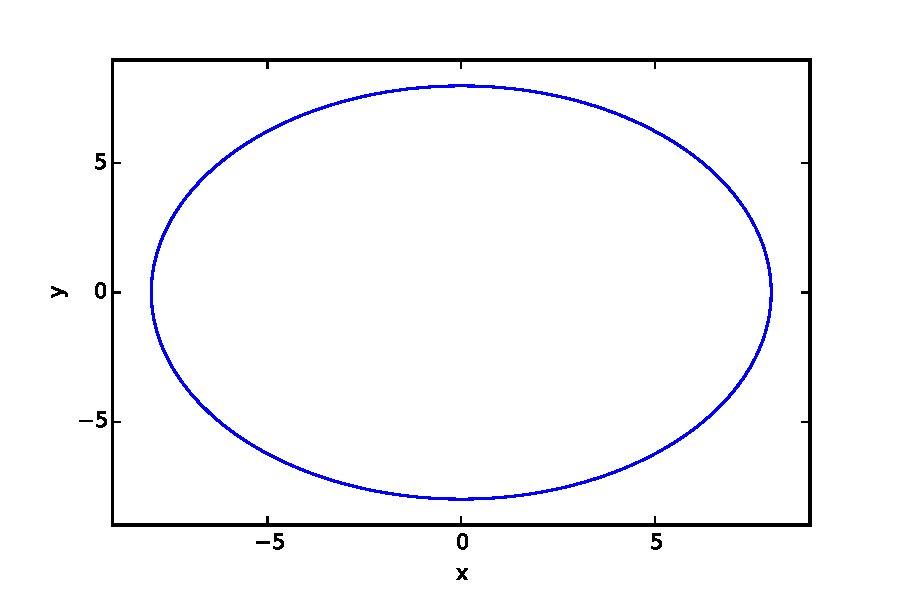
\includegraphics[width=100mm]{pictures/x-y.pdf}
    \caption{Решение задачи о математическом осцилляторе. График зависимости $y(x)$}
    \label{x-y}
\end{figure}
\begin{figure}[H]
\centering
    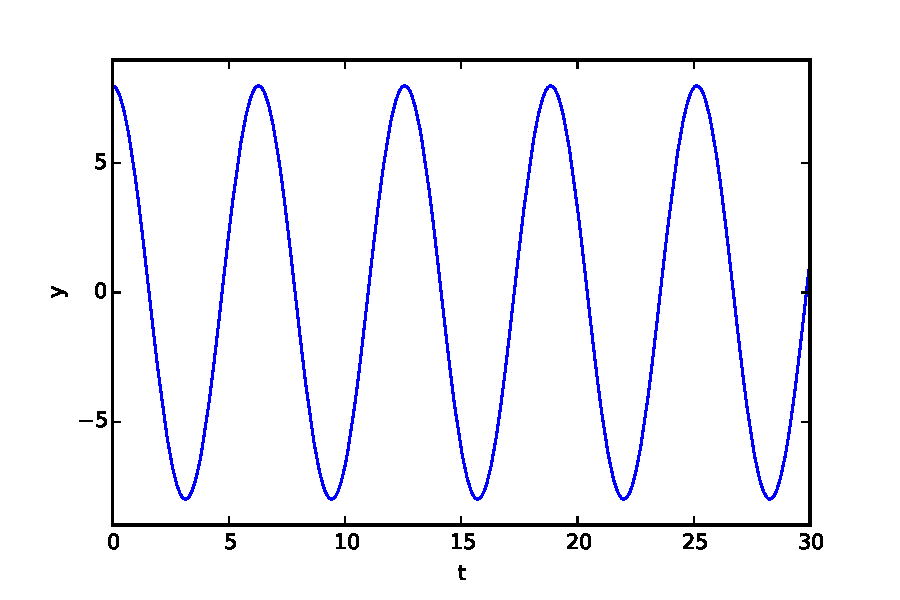
\includegraphics[width=100mm]{pictures/t-y.pdf}
    \caption{Решение задачи о математическом осцилляторе. График зависимости $y(t)$}
    \label{t-y} 
\end{figure}
\begin{figure}[H]
\centering
    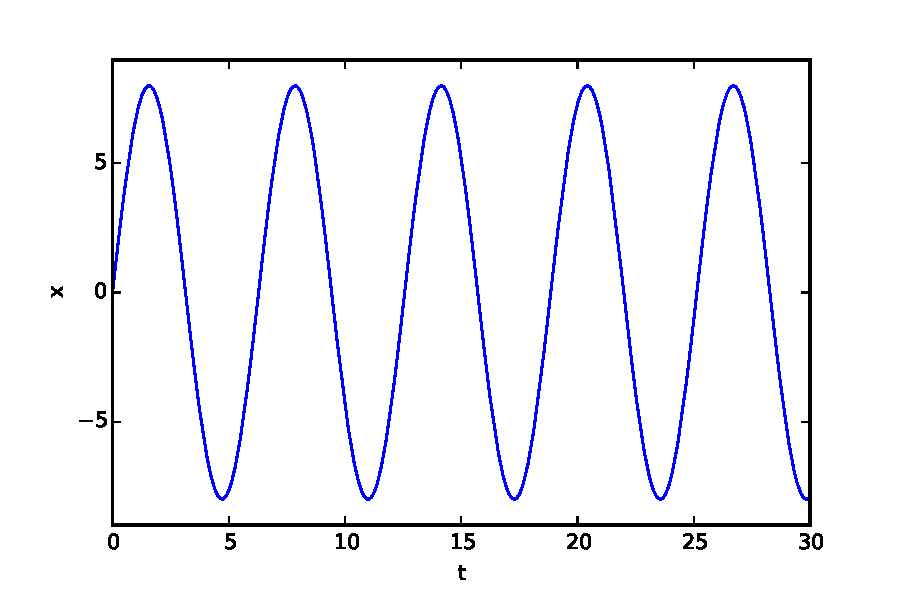
\includegraphics[width=100mm]{pictures/t-x.pdf}
    \caption{Решение задачи о математическом осцилляторе. График зависимости $x(t)$}
    \label{t-x}
\end{figure}

\section{Результаты решения задачи и их анализ}

\section{Cравнение аналитического и численного решений}
\newpage
\begin{thebibliography}{99} 
\bibitem {Grigoriev} 
{\em И.\,С.\,Григорьев.} Методическое пособие по численным методам решения краевых задач принципа 
максимума в задачах оптимального управления \\ Издательство Центра прикладных исследований 
при механико-математическом факультете МГУ, 2005. 
\bibitem {Alexandrov} 
{\em В.\,В.\,Александров, Н.\,С.\,Бахвалов, К.\,Г.\,Григорьев, Г.\,Ю.\,Данков, М.\,И.\,Зеликин, С.\,Я.\,Ищенко, 
С.\,В.\,Конягин, Е.\,А.\,Лапшин, Д.\,А.\,Силаев, В.\,М.\,Тихомиров, А.\,В.\,Фурсиков.} Практикум по 
численным методам в задачах оптимального управления \\ Издательство Московского университета, 1988. 
\bibitem {Zapletin} 
{\em И.\,С.\,Григорьев, И.\,С.\,Заплетин.} Практикум по численным методам в задачах оптимального управления. Дополнение I \\ Издательство Центра прикладных 
исследований при механико-математическом факультете МГУ, 2007. 
\end{thebibliography}

\newpage
\section{Приложения}
\subsection{Решение задачи о математическом осцилляторе в Wolfram Mathematica 9.}
\label{Wolfram}
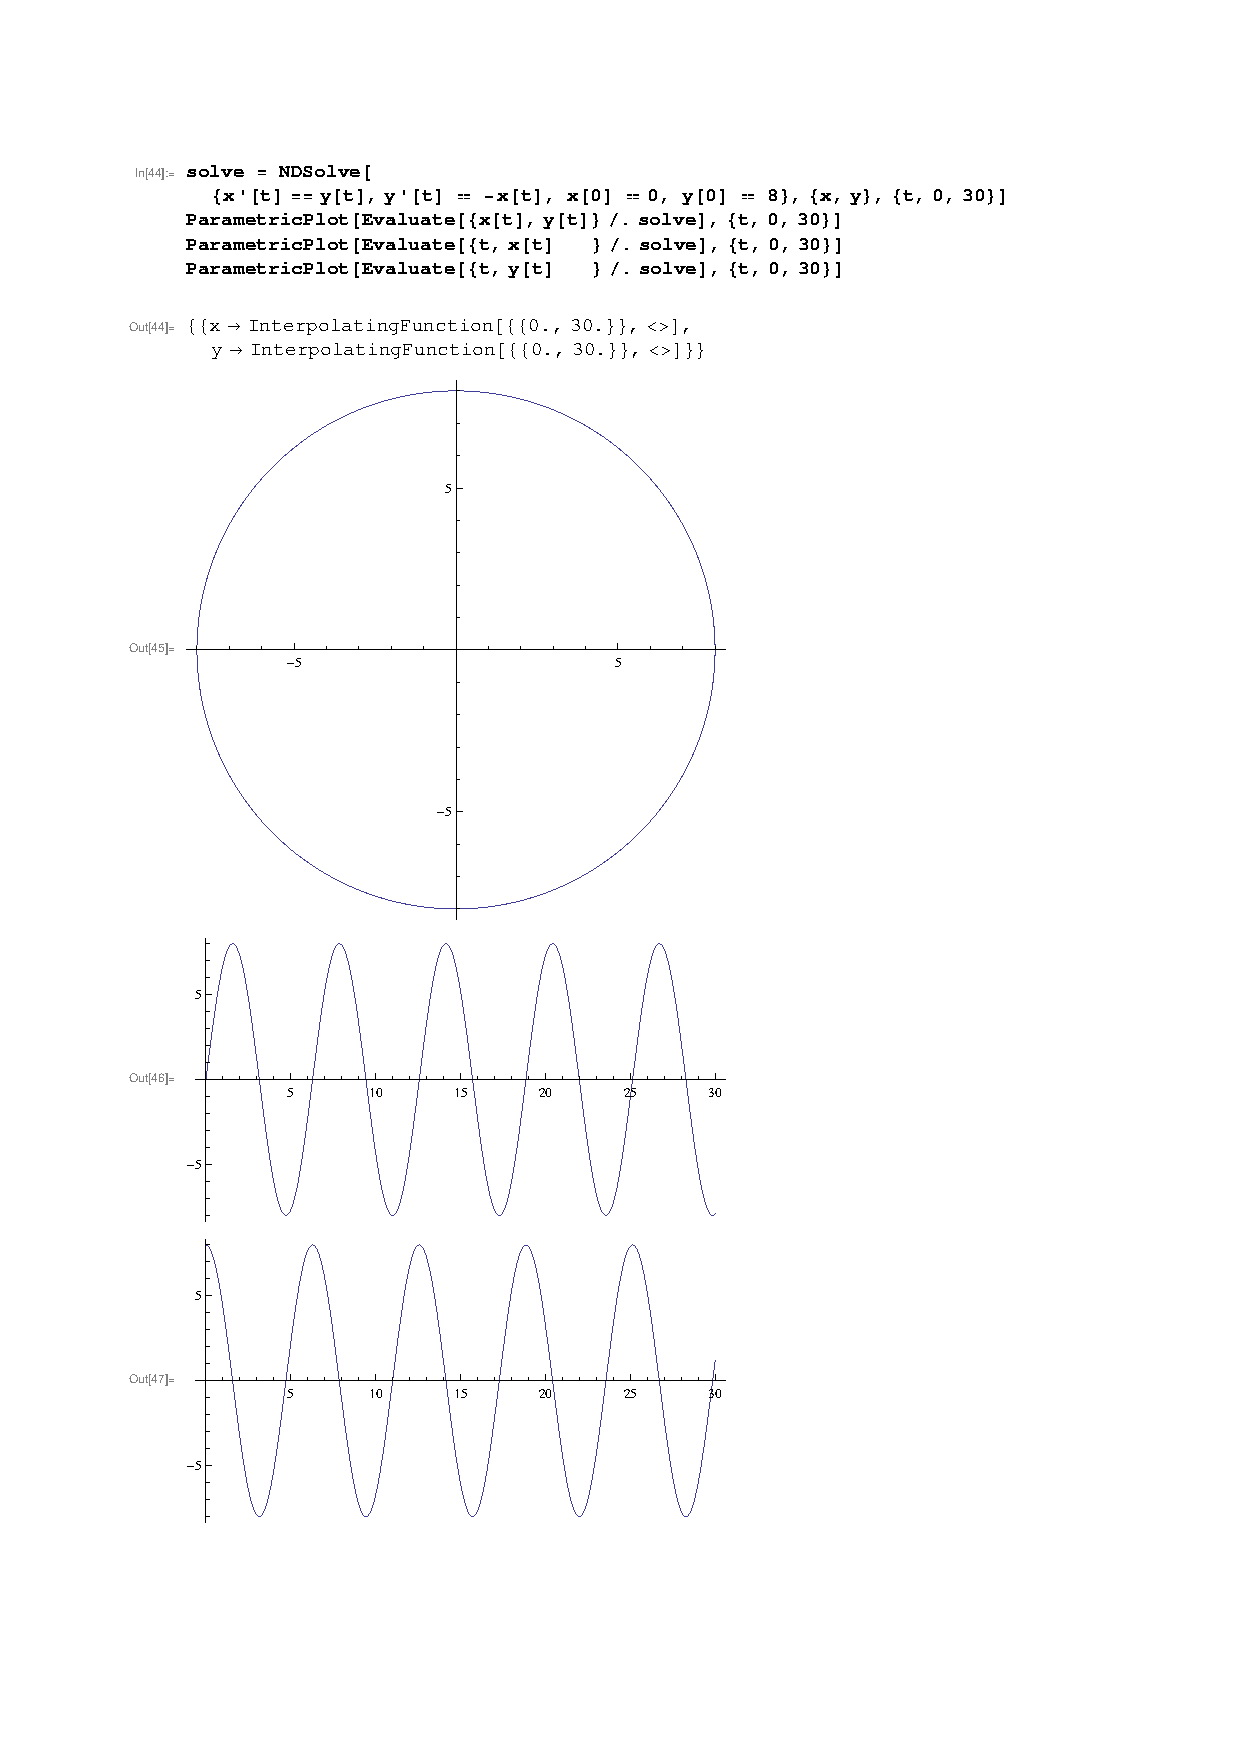
\includepdf[pages={1}]{pictures/oscillator.pdf}

\end{document}